\chapter{Conclusion and Future Research \label{chap_4}}
We have described DELPHI and SPRINT, two bioinformatics programs for predicting PPI biding sites and predicting PPI. Both programs are more accurate than the state-of-the-art methods at the time of the publication. SPRINT is orders of magnitudes faster. 

In this chapter, we discuss some of the common practises in developing bioinformatics tools. We hope these techniques and tips are helpful to others. Then, future research areas are introduced.
\section{Common Deep Learning Practises in Bioinformatics}
As shown in Figure \ref{fig_deep_learning_step}, common deep learning application development steps include defining a problem, preparing data, designing and improving models, and result reporting. Unlike traditional algorithmic approach, most deep learning frameworks such as TensorFlow and PyTorch have a black box design where it is hard to debug line by line. Therefore, the development process is to some level, experience driven; one needs to detect problems by looking at the end results. 
\begin{figure}[h!]
\begin{center}
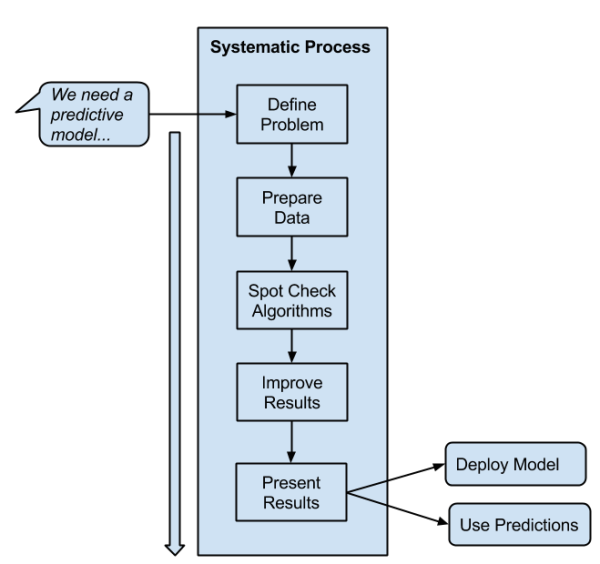
\includegraphics[height=9.5cm]{img/machine_learning_in_bioinf.png}
\caption[Common deep learning application development steps]{Common deep learning application development steps. From machinelearningmastery.com \label{fig_deep_learning_step}}
\end{center}
\end{figure}
\subsection{Data Preparation}
Data preparation is a step often neglected by engineers. Computer scientists tend to focus on the algorithmic aspect of the application, but a trend in deep learning is the increasing importance of having good data. 

Good data has several folds of meanings. First, good training and validation data is the key to train a good model. In general, in deep learning, the more data the better. However, too much data also implies longer training time, so it is also a trade off. Training data should be clean, consistent, and obtained from trustworthy source. Second, several gold standard testing data should be picked at the beginning of the development cycle. Enough attention should be focused on selecting good independent testing dataset. This includes using benchmark testing dataset from previous publications or design your own testing dataset.  Third, data similarities should be checked carefully at the very beginning. The training and validation data should be filtered to contain no similarities to testing data. There should also be no similarities between and among training and validation data. Many high impact publications now require the submitted machine learning manuscripts to have a separate section discussing how training and testing data are dissimilar. Precious time could be wasted if reviewers are concerned about the dataset similarities. Because this could mean revisit the whole development process.

\subsubsection{Comparative Analysis}
To perform comparative analysis, running competing methods is often needed. Sanity check is crucial but often omitted. Sanity check means by executing others' programs, one obtain identical result as reported in previous publications. This ensures running others' program correctly and evaluating result using same way. There are commonly seen mistake due to not having sanity checks. For example, evaluation metrics such as sensitivity, MCC are threshold dependent. That is, the original output of programs are regression values, and a threshold is needed to classify each value into a class, for instance, binding site and non-binding site. All programs should have a uniformed way of selecting the threshold (see Section \ref{sec_evaluation_scheme} as an example). Another common mistake is comparing the evaluation metrics on a complete testing dataset to the average of leave-one-out result on the same testing dataset.

\subsubsection{Improving Results}
After the data is ready, trying different architectures, tuning parameters, and improving results often take several development cycles. It is worthwhile spending time on the infrastructure code. Good code infrastructure, such as scripting, clear system design, makes it easier to change sub-component and try ideas quickly. Following good coding standard and git practise will eventually save time and prevent accumulating technical debt.

Results can be improved by having better data, better features, better model architecture, better regularization (less overfitting). Besides collecting initial training data, sampling and shuffling the data also play a role in obtaining good model. The initial architecture usually comes from literature, and it servers as the baseline performance. Adding new elements that are proven to work in some other field into the baseline model is a good way to improve the performance. For example, ensemble learning and position information are shown to improve performances in areas like image classification and language translation, so modifying and applying them into a bioinformatics problem is also worth trying.

Regularization techniques such as dropout, L1/L2 are critical and effective in reducing model variance. It convenient to parameterize the regularization option in the development code for almost most layers, so we can try many of them quickly.
\section{Future Research}
For PPI sites prediction, many recent published deep learning techniques could potentially further improve the prediction performance. These include better protein sequence embedding using ELMo, the transformer architecture, graph neural network, residual architecture, more sophisticated data sampling. Benchmark data can be improved as well. Three of the testing dataset used in DELPHI are relatively old and new publications are still using them because no better ones exist. The ideas in DELPHI can be also transferred to protein binding sites prediction with other molecules such as DNA, RNA and ligand. Binding-partner specific prediction is also interesting. That is, not only the binding residues are predicted, also the biding proteins. Better features can be potential discovered. Section \ref{sec_arch_fea} shows that the newly added three features are more helpful than the architecture. 

For PPI prediction, our research lab is trying similar deep learning ideas to improve the prediction. The deep learning computational complexity of PPI prediction is higher than site precision. Quantization techniques and mixed precision could be used to accelerate the process. Classifying more specific area of PPI site could also be interesting. For example,  permanent and transient can be predicted separately \cite{perkins2010transient}. 